\documentclass[a4paper, 12pt, openany]{book}

%%% Работа с русским языком % для pdfLatex
\usepackage{cmap}					% поиск в~PDF
\usepackage{mathtext} 				% русские буквы в~фомулах
\usepackage[T2A]{fontenc}			% кодировка
\usepackage[utf8]{inputenc}			% кодировка исходного текста
\usepackage[english,russian]{babel}	% локализация и переносы
\usepackage{indentfirst} 			% отступ 1 абзаца
\usepackage{gensymb}				% мат символы?

%%% Работа с русским языком % для XeLatex
%\usepackage[english,russian]{babel}   %% загружает пакет многоязыковой вёрстки
%\usepackage{fontspec}      %% подготавливает загрузку шрифтов Open Type, True Type и др.
%\defaultfontfeatures{Ligatures={TeX},Renderer=Basic}  %% свойства шрифтов по умолчанию
%\setmainfont[Ligatures={TeX,Historic}]{Times New Roman} %% задаёт основной шрифт документа
%\setsansfont{Comic Sans MS}                    %% задаёт шрифт без засечек
%\setmonofont{Courier New}
%\usepackage{indentfirst}
%\frenchspacing

%%% Дополнительная работа с математикой
\usepackage{amsfonts,amssymb,amsthm,mathtools}
\usepackage{amsmath}
\usepackage{icomma} % "Умная" запятая: $0,2$ --- число, $0, 2$ --- перечисление
\usepackage{upgreek}

%% Номера формул
%\mathtoolsset{showonlyrefs=true} % Показывать номера только у тех формул, на которые есть \eqref{} в~тексте.

%%% Страница
\usepackage{extsizes} % Возможность сделать 14-й шрифт

%% Шрифты
\usepackage{euscript}	 % Шрифт Евклид
\usepackage{mathrsfs} % Красивый матшрифт

%% Свои команды
\DeclareMathOperator{\sgn}{\mathop{sgn}} % создание новой конанды \sgn (типо как \sin)
\DeclareMathOperator{\rg}{\mathop{rg}}
\DeclareMathOperator{\Rg}{\mathop{Rg}}
\DeclareMathOperator{\im}{\mathop{Im}}
\DeclareMathOperator{\tr}{\mathop{tr}}
\DeclareMathOperator{\const}{\mathop{const}}
\DeclareMathOperator{\Id}{\mathop{Id}}
%\DeclareMathOperator{\dim}{\mathop{dim}}
\usepackage{csquotes} % ещё одна штука для цитат
\newcommand{\pd}[2]{\ensuremath{\cfrac{\partial #1}{\partial #2}}} % частная производная
\newcommand{\abs}[1]{\ensuremath{\left|#1\right|}} % модуль
\renewcommand{\phi}{\ensuremath{\varphi}} % греческая фи
\newcommand{\pogk}[1]{\!\left(\cfrac{\sigma_{#1}}{#1}\right)^{\!\!\!2}\!} % для погрешностей


%\renewcommand{\labelenumi}{\asbuk{enumi})}

% Ссылки
\usepackage{color} % подключить пакет color
% выбрать цвета
\definecolor{BlueGreen}{RGB}{49,152,255}
\definecolor{Violet}{RGB}{120,80,120}
% назначить цвета при подключении hyperref
\usepackage[unicode, colorlinks, urlcolor=blue, linkcolor=blue, pagecolor=blue, citecolor=blue]{hyperref} %синие ссылки
%\usepackage[unicode, colorlinks, urlcolor=black, linkcolor=black, pagecolor=black, citecolor=black]{hyperref} % для печати (отключить верхний!)


%% Перенос знаков в~формулах (по Львовскому)
\newcommand*{\hm}[1]{#1\nobreak\discretionary{}
	{\hbox{$\mathsurround=0pt #1$}}{}}

%%% Работа с картинками
\usepackage{graphicx}  % Для вставки рисунков
\graphicspath{{images/}{images2/}}  % папки с картинками
\setlength\fboxsep{3pt} % Отступ рамки \fbox{} от рисунка
\setlength\fboxrule{1pt} % Толщина линий рамки \fbox{}
\usepackage{wrapfig} % Обтекание рисунков и таблиц текстом
\usepackage{multicol}

%%% Работа с таблицами
\usepackage{array,tabularx,tabulary,booktabs} % Дополнительная работа с таблицами
\usepackage{longtable}  % Длинные таблицы
\usepackage{multirow} % Слияние строк в~таблице
\usepackage{caption}
\captionsetup{labelsep=period, labelfont=bf}

%%% Оформление
\usepackage{indentfirst} % Красная строка
%\setlength{\parskip}{0.3cm} % отступы между абзацами
%%% Название разделов
\usepackage{titlesec}
\titlelabel{\thetitle.\quad}
\renewcommand{\figurename}{\textbf{Рис.}}		%Чтобы вместо figure под рисунками писал "рис"
\renewcommand{\tablename}{\textbf{Таблица}}		%Чтобы вместо table над таблицами писал Таблица
\usepackage{enumitem}
\setlist{nolistsep}
\usepackage{verbatim}

%%% Теоремы
\theoremstyle{plain} % Это стиль по умолчанию, его можно не переопределять.
\newtheorem{theorem}{Теорема}[section]
\newtheorem{proposition}[theorem]{Утверждение}
\newtheorem{predlog}{Предложение}[section]
\newtheorem{lemma}{Лемма}[section]

\theoremstyle{definition} % "Определение"
\newtheorem{definition}{Определение}[section]
\newtheorem{corollary}{Следствие}[theorem]
\newtheorem{problem}{Задача}[section]

\theoremstyle{remark} % "Примечание"
\newtheorem*{nonum}{Решение}
\newtheorem{zamech}{Замечание}[theorem]

%%% Правильные мат. символы для русского языка
\renewcommand{\epsilon}{\ensuremath{\varepsilon}}
\renewcommand{\phi}{\ensuremath{\varphi}}
\renewcommand{\kappa}{\ensuremath{\varkappa}}
\renewcommand{\le}{\ensuremath{\leqslant}}
\renewcommand{\leq}{\ensuremath{\leqslant}}
\renewcommand{\ge}{\ensuremath{\geqslant}}
\renewcommand{\geq}{\ensuremath{\geqslant}}
\renewcommand{\emptyset}{\varnothing}

%%% Для лекций по инфе
\usepackage{alltt}
\newcounter{infa}[section]
\newcounter{num}
\definecolor{infa}{rgb}{0, 0.2, 0.89}
\definecolor{infa1}{rgb}{0, 0.3, 1}
\definecolor{grey}{rgb}{0.5, 0.5, 0.5}
\newcommand{\tab}{\ \ \ }
\newcommand{\com}[1]{{\color{grey}\##1}}
\newcommand{\num}{\addtocounter{num}{1}\arabic{num}\tab}
\newcommand{\defi}{{\color{infa}def}}
\newcommand{\ini}{{\color{infa}in}}
\newcommand{\rangei}{{\color{infa}range}}
\newcommand{\fori}{{\color{infa}for}}
\newcommand{\ifi}{{\color{infa}if}}
\newcommand{\elsei}{{\color{infa}else}}
\newcommand{\printi}{{\color{infa1}print}}
\newcommand{\maxi}{{\color{infa}max}}
\newcommand{\classi}{{\color{infa}class}}
\newcommand{\returni}{{\color{infa}return}}
\newcommand{\elifi}{{\color{infa}elif}}


\newenvironment{infa}[1]{
	
	\vspace{0.5cm}
	\addtocounter{infa}{1}%
	\noindent{\large \textbf{Программа №\thesection.\arabic{infa}}}\textbf{<<#1>>}%
	\begin{alltt}%
	}{\end{alltt}
	\setcounter{num}{0}
	\vspace{0.1cm}}
%Пример кода:
%\begin{infa}{Поразрядная сортировка}
%	\ \num \defi count_sort(a):\tab \com{определяет нашу функцию}
%	\ \num \tab m = \maxi(a)+1
%	\ \num \tab q = [0]*m
%	\ \num \tab \fori x \ini a:
%	\ \num \tab \tab q[x] += 1
%	\ \num \tab pos = 0
%	\ \num \tab \fori x \ini q:
%	\ \num \tab \tab \fori i \ini \rangei(q[x]):
%	\ \num \tab \tab \tab a[pos] = x
%	\num \tab \tab \tab pos += 1
%\end{infa}

\usepackage{titlesec}
\titlelabel{\thetitle.\quad}

\usepackage{biblatex}
\addbibresource{references.bib}

\usepackage[left=1.27cm,right=1.27cm,top=2cm,bottom=2cm]{geometry}

\usepackage{fancyhdr} % Для колонтитулов

\renewcommand{\baselinestretch}{1.3}

\makeatletter % Убирает нумерацию на страницах, где \chapter
\renewcommand\chapter{\if@openright\cleardoublepage\else\clearpage\fi
	\thispagestyle{empty}% original style: plain
	\global\@topnum\z@
	\@afterindentfalse
	\secdef\@chapter\@schapter}
\makeatother

\usepackage{fancyhdr}
\pagestyle{fancy}
\fancyhf{}
\fancyhead[L]{\rightmark}
\fancyhead[R]{\textbf{\thepage}}

\setcounter{secnumdepth}{0}

\newcommand\invisiblesection[1]{%
	\refstepcounter{section}%
	\addcontentsline{toc}{section}{#1}%
	\sectionmark{#1}}


\title{Вопрос по выбору}
\author{Алексей Кожарин}
\date{today}
\usepackage[left=1.27cm,right=1.27cm,top=2cm,bottom=2cm]{geometry}

\usepackage{fancyhdr} % Для колонтитулов

\renewcommand{\baselinestretch}{1.3}

\makeatletter % Убирает нумерацию на страницах, где \chapter
\renewcommand\chapter{\if@openright\cleardoublepage\else\clearpage\fi
	\thispagestyle{empty}% original style: plain
	\global\@topnum\z@
	\@afterindentfalse
	\secdef\@chapter\@schapter}
\makeatother

\usepackage{fancyhdr}
\pagestyle{fancy}
\fancyhf{}
\fancyhead[L]{\rightmark}
\fancyhead[R]{\textbf{\thepage}}

\setcounter{secnumdepth}{0}

\newcommand\invisiblesection[1]{%
	\refstepcounter{section}%
	\addcontentsline{toc}{section}{#1}%
	\sectionmark{#1}}

\begin{document}
	
	\invisiblesection{Отрицательная статистическая температура}
	\section{Определение}
	\hspace{0.4cm}\textbf{Отрицательная абсолютная температура} — температура, характеризующая равновесные состояния термодинамической системы, в которых вероятность обнаружить систему в микросостоянии с более высокой энергией выше, чем в микросостоянии с более низкой.
	В классической статистике этому соответствует большая плотность вероятности для точек фазового пространства с более высокой энергией по сравнению с точками с более низкой энергией. При положительной температуре соотношение вероятностей или их плотностей обратное.
	
	\tab Отрицательная температура системы сохраняется достаточно долго, если эта система достаточно хорошо изолирована от тел с положительной температурой. На практике отрицательная температура может реализовываться, например, в системе ядерных спинов.
	
	\tab При этом абсолютная температура $+\infty$ и $-\infty$  — это одна и та же температура (соответствующая равномерному распределению), но различаются температуры $T=+0$ и $T=-0$ . Так, система будет сосредоточена на самом нижнем уровне при $T=+0$ , и на самом верхнем — при $T=-0$ .
	
	\section{Инверсия заселенностей}
	В случае термодинамического равновесия, состояние с низкой энергией намного популярней возбуждённого состояния, и это является нормальным состоянием системы. Если удастся каким-либо способом \textit{обратить} ситуацию, то тогда говорят, что система перешла в состояние с \textbf{инверсией электронных заселенностей}.\\
	Из распределения Больцмана для отношения числа молекул на двух уровнях:
	\begin{equation}
		\cfrac{N_2}{N_1}=\exp \cfrac{-(E_2-E_1)}{kT}
		\label{otn}
	\end{equation}
	Если при $E_2 > E_1$ нам удастся достичь такое состояние, что $N_2 > N_1$, то из формулы \ref{otn} получим, что $ T < 0 $. Существует несколько моделей, реализующих данное состояние.
	
	\tab Рассмотрим одну из таких моделей, известную как трёхуровневый лазер. Возьмем группу из $N$ атомов так, что каждый из них может находиться в трёх различных энергетических состояниях, на уровнях 1, 2 и 3 с энергиями $E_1$, $E_2$ и $E_3$, в количестве $N_1$, $N_2$ и $N_3$, соответственно. При этом диаграмма энергетических уровней будет выглядеть следующим образом:
	\begin{figure}[h]
		\center{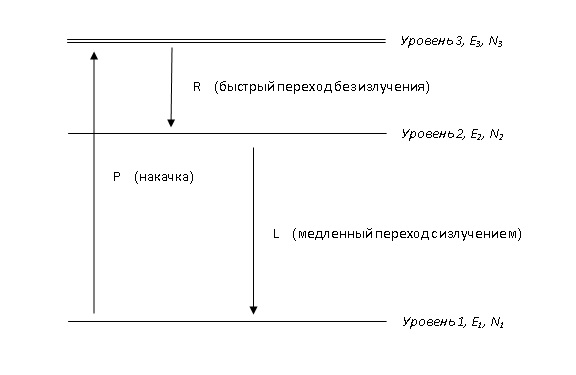
\includegraphics[width=0.85\linewidth]{diag1}}
		\caption{
			Диграмма энергетических уровней (трехуровневый лазер).
		}
		\label{diag1}
	\end{figure}
	\newpage
	На этой диаграмме $E_1 < E_2 < E_3$; т. е. энергетический уровень 2 лежит между основным состоянием и уровнем 3.
	
	В самом начале система атомов находится в термодинамическом равновесии и большинство атомов находится в основном состоянии, т. е. $N_1 \approx N, N_2 \approx N_3 \approx 0$. Если теперь осветить атомы светом частоты $\nu_{31}$, где $E_3 - E_1 = h\nu_{31}$ ($h$ — Постоянная Планка), благодаря поглощению, начнётся процесс перехода атомов в возбуждённое состояние на уровень 3. Такой процесс называется накачкой, и не всегда он вызывается светом. Для этой цели также применяются электрические разряды или химические реакции.
	
	Если мы будем продолжать накачку атомов, мы возбудим до уровня 3 достаточное их количество, т. е. $N_3 > 0$. Далее нам необходимо, чтобы атомы быстро перешли на уровень 2. Освобождённая при этом энергия может излучиться в виде фотона механизмом спонтанного излучения, но на практике рабочее тело лазера выбирают так, чтобы переход $3 \rightarrow 2$, обозначенный на диаграмме буквой \textbf{R}, проходил без излучения, а энергия тратилась на нагрев рабочего тела.
	
	Атом на уровне 2 может перейти на основной уровень, спонтанно излучив фотон частоты $\nu_{21}$ (которую можно найти из выражения $E_2-E_1 = h\nu_{21}$). Этот процесс показан на диаграмме буквой \textbf{L}. Время до этого перехода $\tau_{21}$ значительно превышает время неизлучающего перехода $3 \rightarrow 2$ — $\tau_{32} (\tau_{21} \gg \tau_{32}$). При таком условии количество атомов на уровне 3 будет примерно равно нулю ($N_3 \approx 0$), а количество атомов на уровне 2 — больше нуля ($N_2 > 0$), поскольку переход $2 \rightarrow 1$ будет определять всю скорость перехода $3 \rightarrow 1$. Если на уровне 2 удастся удержать больше половины атомов, между уровнями 1 и 2 будет достигнута инверсия населённостей.
	
	Поскольку для достижения такого эффекта нужно возбудить не менее половины атомов, для накачки нужна очень большая энергия. Поэтому трёхуровневые лазеры непрактичны, хотя они и стали первыми созданными Теодором Майманом лазерами (на основе рубина) в 1960 году. На практике чаще используются четырёхуровневые лазеры, как показано на диаграмме ниже:
	\begin{figure}[h]
		\center{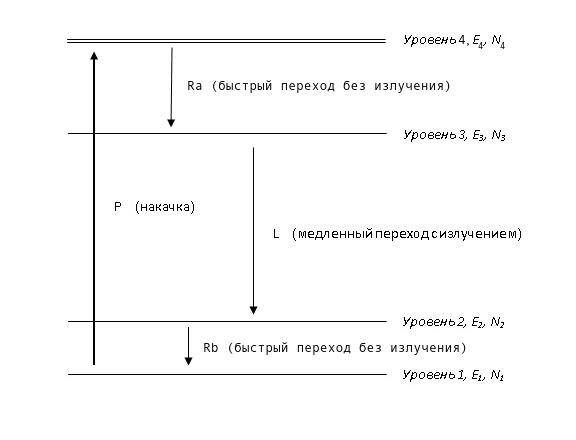
\includegraphics[width=0.85\linewidth]{diag2}}
		\caption{
			Диаграмма для четырехуровневого лазера.
		}
		\label{diag2}
	\end{figure}
	
	Здесь присутствует четыре энергетических уровня $E_1$, $E_2$, $E_3$, $E_4$, и количество атомов $N_1$, $N_2$, $N_3$, $N_4$, соответственно. Энергии этих уровней последовательно увеличиваются: $E_1 < E_2 < E_3 < E_4$.
	
	В такой системе при накачке \textbf{P} атомы переходят из основного состояния (уровень 1) на уровень накачки 4. С уровня 4 атомы с помощью быстрого неизлучающего перехода \textbf{Ra} — на уровень 3. Так как время до перехода \textbf{L} намного превышает время до перехода \textbf{Ra}, на уровне 3 скапливаются атомы, которые затем с помощью спонтанного или вынужденного излучения переходят на уровень 2. С этого уровня быстрым переходом \textbf{Rb} атом может вернуться в основное состояние.
	
	Как и в предыдущем случае, наличие быстрого перехода \textbf{Ra} приводит к тому, что $N_4 \approx 0$. В четырёхуровневом лазере, благодаря наличию второго быстрого перехода \textbf{Rb}, количество атомов на уровне 2 также стремится к нулю ($N_2 \approx 0$). Это значительно упрощает достижение инверсии заселенностей.
	
	Полученное оптическое усиление (и, соответственно, работа лазера) происходит на частоте $\nu_{32}$ ($E_3-E_2 = h\nu_{32}$). Так как для образования инверсии населённостей в четырёхуровневом лазере достаточно небольшого числа атомов, такие лазеры более практичны.
	
\end{document}